\section{Exercise 5}

Consider the C program below:
\begin{verbnobox}[\verbarg]
#include <stdio.h>
#include <stdlib.h>
#include <string.h>
#include <unistd.h>
#include <fcntl.h>

typedef struct {
    char username[40];
    char password[20];
} user_t;

void welcome_user(user_t * user){
    char message[52];
    strcpy(message, "Ciao to "); // len 8
    strcat(message, user->username); // len 8+40
    strcat(message, "\n"); // len 8+40+1 == 49 < 52, ok
    printf(message);
    return;
}

int main() {
    user_t user;

    printf("Insert your name: ");
    read(0, user.username, 40); // 0 == stdin
    printf("Insert your password: ");
    read(0, user.password, 20); // 0 == stdin

    welcome_user(&user);

return 0;
}
\end{verbnobox}
\begin{enumerate}
    \item The program is affected by a typical buffer overflow. 
        Find the line affected and describe the reason. 
    \item Focus only on the stack-based buffer overflow(s) you found. 
        Write an exploit for this vulnerability that must execute the following shell code, composed of eight bytes, which opens a shell: \texttt{0x20 0x30 0x40 0x50 0x60 0x70 0x80 0x90}.
        Describe all the steps and assumptions required to successfully exploit the vulnerability. 
        Include also any assumption on how you must call and run the program: e.g., the values for the command-line arguments required to trigger the exploit correctly and/or environment variables (if any), the input provided during the execution, if multiple executions are necessary. 
    \item Make sure that you show how the exploit will appear in the process memory with respect to the stack layout right before and after the execution of the vulnerable line during the program exploitation showing:
    \begin{itemize}
        \item Direction of growth and high-low addresses. 
        \item The name of each allocated variable. 
        \item The content of relevant registers (i.e., EBP, ESP). 
        \item The functions stack frames.
    \end{itemize}
    Show also the content of the caller frame. 
\end{enumerate}

\subsection*{Solution}
\begin{enumerate}
    \item A buffer overflow occurs at line fourteen because \texttt{strcat} concatenates strings until the first null terminator \texttt{/0}.
        If the \texttt{username} doesn't contain a \texttt{/0}, \texttt{strcat} will copy the \texttt{password} as well.
    \item We can fill \texttt{user.username} with a NOP sled and the shell code, totaling 40 non-zero bytes. 
        Then, we place the desired return address inside \texttt{user.password}.
        \begin{verbatim}
user.username = "\x90\x90\x90" + ... + shell code
user.password = "A"*8 + target_address
        \end{verbatim}
    \item The stack with the exploit applied is depicted below:
        \begin{figure}[H]
            \centering
            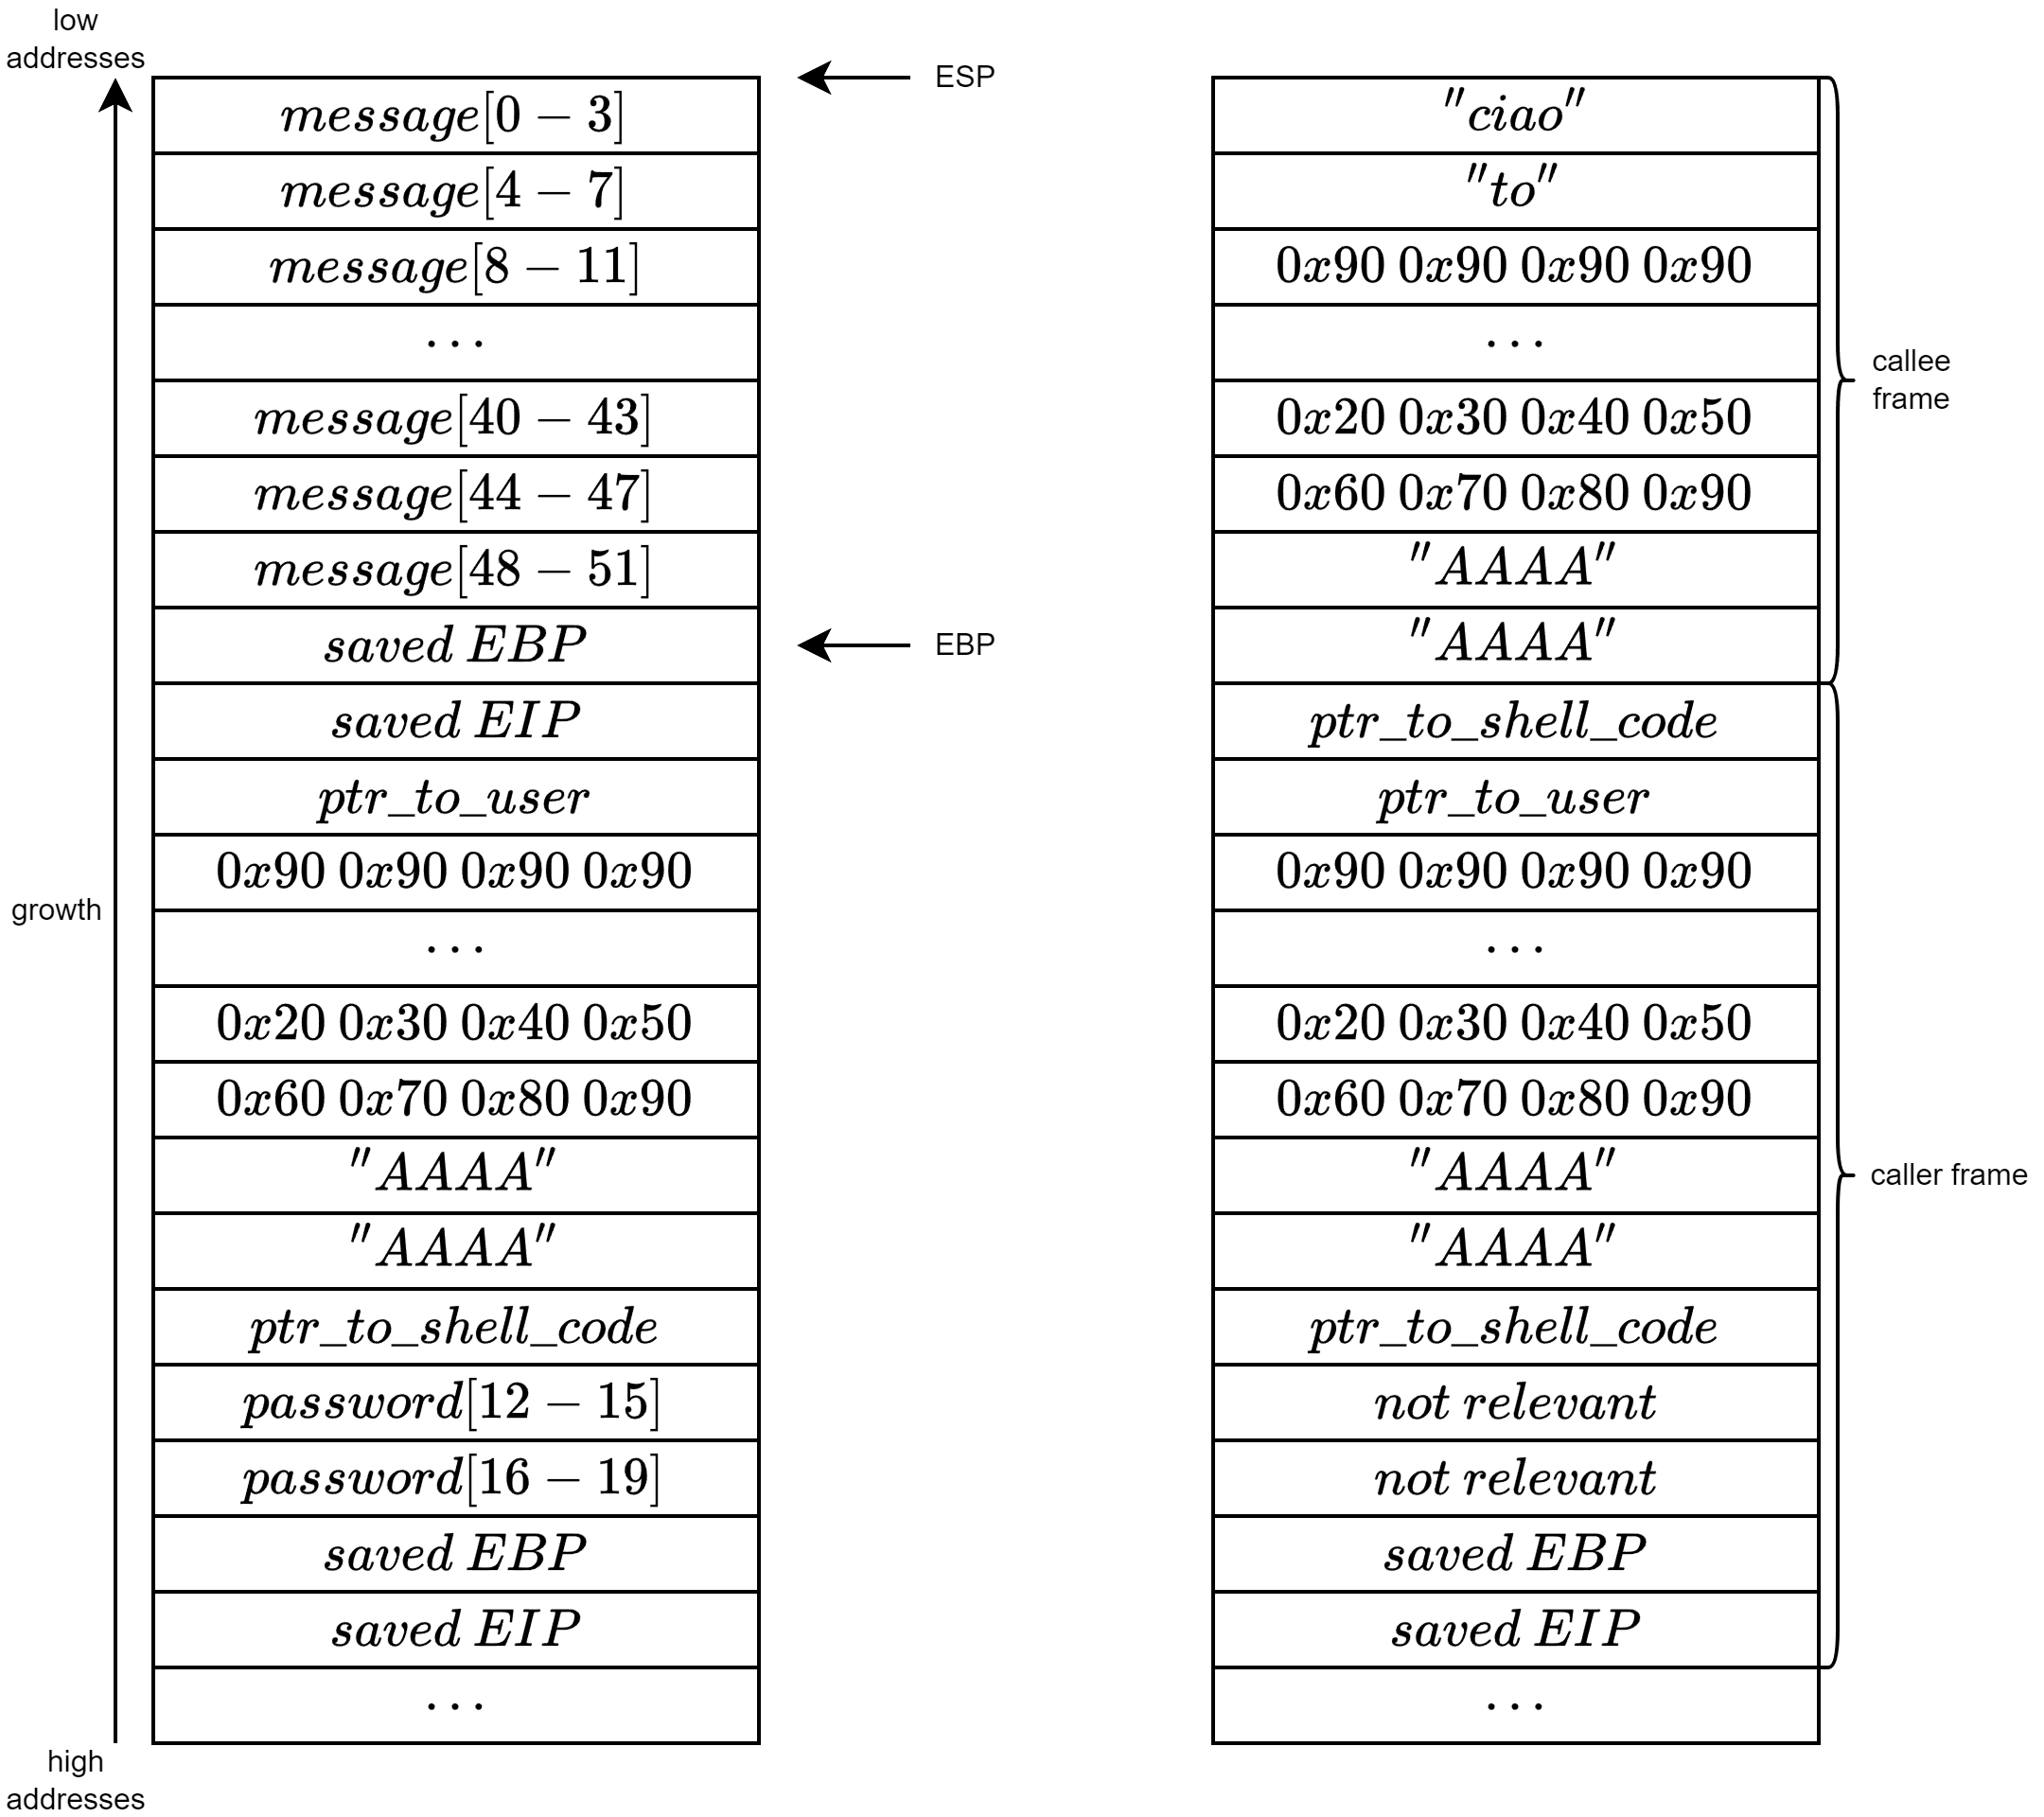
\includegraphics[width=0.75\linewidth]{images/stack8.png}
        \end{figure}
\end{enumerate}